\documentclass[a4paper, 12pt]{article}

%%% Работа с русским языком
\usepackage{cmap}					% поиск в PDF
\usepackage{mathtext} 				% русские буквы в формулах
\usepackage[T2A]{fontenc}			% кодировка
\usepackage[utf8]{inputenc}			% кодировка исходного текста
\usepackage[russian]{babel}	% локализация и переносы

%%% Дополнительная работа с математикой
\usepackage{amsmath,amsfonts,amssymb,amsthm,mathtools} % AMS
\usepackage{icomma} % "Умная" запятая: $0,2$ --- число, $0, 2$ --- перечисление

%% Номера формул
%\mathtoolsset{showonlyrefs=true} % Показывать номера только у тех формул, на которые есть \eqref{} в тексте.
%\usepackage{leqno} % Немуреация формул слева

%% Шрифты
\usepackage{euscript}	 % Шрифт Евклид
\usepackage{mathrsfs} % Красивый матшрифт

%%% Свои команды
\DeclareMathOperator{\sgn}{\mathop{sgn}}

%% Поля
\usepackage[left=2cm,right=2cm,top=2cm,bottom=2cm,bindingoffset=0cm]{geometry}

%% Русские списки
\usepackage{enumitem}
\makeatletter
\AddEnumerateCounter{\asbuk}{\russian@alph}{щ}
\makeatother

%%% Работа с картинками
\usepackage{graphicx}  % Для вставки рисунков
\graphicspath{{images/}{images2/}}  % папки с картинками
\setlength\fboxsep{3pt} % Отступ рамки \fbox{} от рисунка
\setlength\fboxrule{1pt} % Толщина линий рамки \fbox{}
\usepackage{wrapfig} % Обтекание рисунков и таблиц текстом

%%% Работа с таблицами
\usepackage{array,tabularx,tabulary,booktabs} % Дополнительная работа с таблицами
\usepackage{longtable}  % Длинные таблицы
\usepackage{multirow} % Слияние строк в таблице

%% Красная строка
\setlength{\parindent}{2em}

%% Интервалы
\linespread{1}
\usepackage{multirow}

%% TikZ
\usepackage{tikz}
\usetikzlibrary{graphs,graphs.standard}

%% Верхний колонтитул
\usepackage{fancyhdr}
\pagestyle{fancy}

%% Перенос знаков в формулах (по Львовскому)
\newcommand*{\hm}[1]{#1\nobreak\discretionary{}
	{\hbox{$\mathsurround=0pt #1$}}{}}

%% дополнения
\usepackage{float} % Добавляет возможность работы с командой [H] которая улучшает расположение на странице
\usepackage{gensymb} % Красивые градусы
\usepackage{caption} % Пакет для подписей к рисункам, в частности, для работы caption*

% подключаем hyperref (для ссылок внутри  pdf)
\usepackage[unicode, pdftex]{hyperref}

%%% Теоремы
\theoremstyle{plain}                    % Это стиль по умолчанию, его можно не переопределять.
\renewcommand\qedsymbol{$\blacksquare$} % переопределение символа завершения доказательства

\newtheorem{theorem}{Теорема}[section] % Теорема (счетчик по секиям)
\newtheorem{proposition}{Утверждение}[section] % Утверждение (счетчик по секиям)
\newtheorem{definition}{Определение}[section] % Определение (счетчик по секиям)
\newtheorem{corollary}{Следствие}[theorem] % Следстиве (счетчик по теоремам)
\newtheorem{problem}{Задача}[section] % Задача (счетчик по секиям)
\newtheorem*{remark}{Примечание} % Примечание (можно переопределить, как Замечание)
\newtheorem{lemma}{Лемма}[section] % Лемма (счетчик по секиям)

\newtheorem{example}{Пример}[section] % Пример
\newtheorem{counterexample}{Контрпример}[section] % Контрпример

\begin{document}
    \newcommand{\HRule}{\rule{\linewidth}{0.7mm}} % Defines a new command for the horizontal lines, change thickness here
	
	\begin{center}
		\large\textbf{Московский Физико-Технический Институт}\\ % Name of your university/college
		\large\textbf{(государственный университет)}
	
		\vfill
		
		\Large Научный проект по защите информации\\[0.5cm] % Preambule of your document title
		
		
		\HRule
		\\[0.4cm]
		{ \huge \bfseries *Реализация шифра <<Кузнечик>> с применением векторных инструкций RISC-V архитектуры*} % Title of your document
		\\[0.4cm]
		\HRule
		\\[0.5cm]
		
		\ \\
	\textbf{\large Авторы:} \\
	\large Филиппенко Павел Б01-009\\
        \large Фролов Даниил Б01-009\\
        \large Долгодворов Егор Б01-009\\
        \large Белов Владислав Б01-009\\
		\vfill
		\hspace*{-0.8 cm}
\includegraphics[width=100 pt]{../images/frkt_logo}\\ % Logo of your  company/university/college
		\large Долгопрудный, 2023 % Location and year
	\end{center}

\newpage
\setcounter{page}{2}
\fancyfoot[c]{\thepage}
\fancyhead[L] {Криптография} % Information in page header
\fancyhead[R]{}

    \section{Abstract}
    Для современных компьютерных систем важно, чтобы алгоритмы шифрования данных были не
    только надежными, но и быстрыми с точки зрения вычислительных операций. В
    данной статье мы реализуем алгоритм блочного шифрования с использованием векторного
    расширения RISC-V на примере шифра ГОСТ 34.12-2015 <<Кузнечик>>. Сравним производительности последовательной и векторизованной реализаций.

    \section{Введение}

    В современном мире, где значительную роль играют цифровые технологии,
    криптография является основной составляющей обеспечения безопасности в цифровой
    среде: защита интернет-соединений и каналов связи, надежность проведения банковских
    операций, подтверждение подлинности электронных документов. Современные методы
    защиты информации накладывают большое количество требований на современные 
    алгоритмы шифрования, такие как теоретическая и вычислительная криптостойкость, а 
    также скорость работы.
    
    Существует множество различных методик повышения производительности алгоритмов. На 
    сегодняшний день одним из распространенных способов увеличения скорости работы программ является векторизация скалярных операций. Данный способ основывается на 
    принципе компьютерных вычислений SIMD (англ. single instruction multiple data), 
    позволяющем обеспечить параллелизм на уровне данных. Несмотря на то, что данный вид
    оптимизации требует индивидуальной реализации для разных архитектур, он является
    довольно эффективным методом увеличения производительности кода. Кроме того, векторизацию удобно использовать в алгоритмах с большим количеством однотипных математических
    операций, в частности, в алгоритмах блочного шифрования.

    В данной статье мы предложим векторную реализацию блочного шифра <<Кузнечик>> для 
    процессорной архитектуры RISC-V, а также сравним скорость работы
    последовательной и векторизованной реализаций.

    \section{Шифр <<Кузнечик>>}

    Алгоритм шифрования <<Кузнечик>> является одним из двух шифров, принятых в 2015 г.
    в России в стандарт блочного шифрования ГОСТ Р 34.12-2015. <<Кузнечик>> относится
    к типу блочных симметричных шифров; это значит, что для зашифрования и
    расшифрования используется один и тот же ключ и что при шифровании исходный текст
    разделяется на блоки фиксированной длины, каждый из которых шифруется отдельно.

    \section{Математическое описания шифра <<Кузнечик>>}

    %%TODO: write this sections
    % \subsection{SP-сети}

    % \subsection{Ячейка Фейстеля}

    \subsection{<<Кузнечик>>}

    Непосредственно алгоритм шифрования <<Кузнечик>> основан на SP-сети, а не на ячейке 
    Фейстеля. Как и другие распространенные шифры, <<Кузнечик>> является блочным итеративным 
    шифром, а это значит, что для каждой итерации необходимо генерировать отдельный 
    \textbf{итеративный ключ} на основе исходного \textbf{мастер-ключа}. Здесь и
    нашла свое применение \textbf{ячейка Фейстеля}. Принцип ячейки Фейстеля используется
    для генерации итеративных ключей.

    Подведем промежуточный итог -- обозначим последовательность действий в алгоритме 
    шифрования:

    \begin{enumerate}
        \item На вход алгоритма подается исходный открытый текст $M$.
%TODO:  Этот текст разбивается на блоки $M_i$ по 128 бит
        \item Этот текст разбивается на блоки по 128 бит $M_i$ (если размер исходного текста не кратен $128$, то он дополняется до нужного размера с помощью заранее оговоренной последовательности).
        \item Полученные блоки обрабатываются итеративно. После обработки всех блоков исходного текста, мы получаем набор блоков шифротекста $C_i$.
        \item Полученные блоки шифротекста объединяются с помощью заранее обговоренного алгоритма (об этом будет сказано дальше), формируя итоговый шифротекст $C$.
    \end{enumerate}

    Распишем более подробно этап итеративной обработки каждого блока и приведем
    набор действий, производящихся с одним блоком в каждой итерации.

    \begin{enumerate}
        \item На вход поступает блок открытого текста $M_i$ длинной 128 бит.
        \item Для текущей итерации с помощью ячейки Фейстеля генерируется раундовый ключ $K_i$ длинной $128$ бит.
        \item Блок исходного текста и раундовый ключ складываются по модулю $2$, образуя новый блок длинной $128$ бит $B_i = M_i \oplus K_i$.
        \item К полученному блоку применяется затем нелинейное преобразование $S$, а затем линейное преобразование $L$, таким образом, получается блок шифротекста $C_i = L(S(B_i)) = L(S(M_i \oplus K_i))$.
    \end{enumerate}

    Блок-схема одной итерации, производящейся с блоком данных приведена на рис. \ref{fig:AlgorithBlockScheme}.

    \begin{figure}
        \centering
        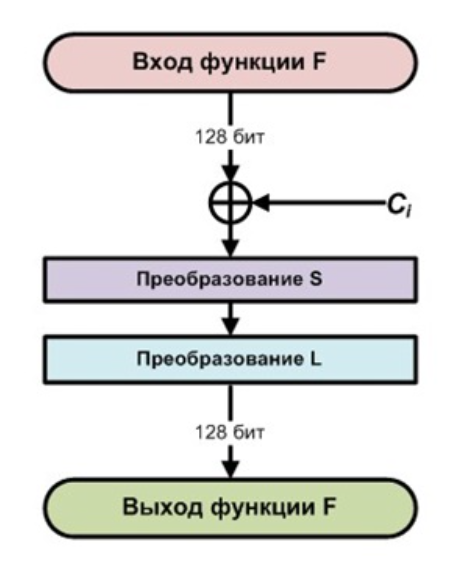
\includegraphics{images/AlgorithBlockScheme.png}
        \caption{Один раунд шифрования в алгоритме <<Кузнечик>>}
        \label{fig:AlgorithBlockScheme}
    \end{figure}

    Опишем теперь суть нелинейного преобразования $S$ и линейного 
    преобразования $L$.

    \subsubsection{Нелинейное S-преобразование}

    На вход нелинейному преобразованию поступает блок данных длинной $128$ бит. Этот блок
    делится на $16$ частей по $8$ бит. Каждая $8$-битовая часть интерпретируется как целое число $UInt_8$, назовем его $a$. 

    \begin{proposition} \label{propos:a_is_8_bit}
    Число $a$ будет находиться в диапазоне от $0$ до $255$, поскольку является $8$-битным 
    беззнаковым числом в двоичной записи.
    \end{proposition}

    В шифрующем алгоритме хранится заранее подготовленный массив из $256$ констант. Каждое
    число $a$ выступает в качестве индекса в этом массиве. Значение по этому индексу преобразуется обратно в двоичное 
    число и является результатом работы блока нелинейного преобразования $S$.

    Приведем пример. \textbf{Внимание! Для удобства читателя в примерах все математические операции выполняются над полем целых чисел. В реальном алгоритме шифрования математические операции проводятся в поле Галуа $\mathbf{GF}(2^8)$ с модулем $p(x) = x^8 + x^7 + x^6 + x + 1$. В таком поле сложение производится по модулю 2, а умножение по модулю многочлена $p(x)$}

    %TODO: дописать пример
    \begin{example}

    Для удобства в этом примере будем считать, что на вход нелинейного преобразования
    поступает блок $16$ бит, который делится на $4$ части по $4$ бита.
    
    \end{example}

    \subsubsection{Линейное L-преобразование}

    Линейное преобразование $L$ представляет собой $16$ последовательных применений более
    простого линейного преобразования $R$, таким образом $L = R^{16}$. Можно подумать,
    что это бессмысленная операция, так как $16$ последовательных линейных
    преобразований можно привести к одному применению линейного преобразования с 
    соответствующими коэффициентами.

    \begin{example}
        Пусть $f_1(x) = k_1 x + b_1$ и $f_2(x) = k_2 x + b_2$. Пусть $y = f_1(f_2(x))$,
        тогда можно последовательное применений функций $f_1$ и $f_2$ заменить 
        применением одной линейной функции $F = K x + B$, где $K = k_1 k_2$ и $B = k_1 b_2 + b_1$.
    \end{example}

    Однако, в нашем случае все немного сложнее, подход $L = R^{16}$ имеет смысл по 
    следующей причине: линейное преобразование $R$ представляет блок входных данных
    длинной $128$ бит, как $16$ $8$-битных чисел, которые, в свою очередь, являются начальными
    значениями регистра сдвига. Далее, начальные значения регистра сдвига умножаются на 
    $16$ заранее известных констант и складыватся, образуя новое значение ячейки регистра 
    сдвига. После $16$ итераций в ячейках регистра сдвига мы получим $16$ новых чисел, 
    которые представляются в бинарном виде и вместе образуют $128$ бит выхода линейного
    преобразования $L$.

    Приведем пример.

    %TODO: дописать пример
    % \begin{example}
        
    % \end{example}
    
    \section{RISC-V}

    \subsection{Мотивация}

    \textbf{RISC-V} ~---~ расширяемая и открытая система команд, а также процессорная архитектура
    на основе концепции \textbf {RISC}\footnote{Концепция RISC заключается в малом количестве инструкций
    архитектуры, что позволяет ускорить расшифрование инструкций и исполнение всей программы в целом.}.
    RISC-V архитектура появилась лишь в 2010 году и является одной из самых перспективных тем для изучения. Основными преимуществами RISC-V архитектуры являются:

    \begin{enumerate}
        \item \textbf{Простота.} Как уже было сказано ранее, RISC-V подчиняется философии RISC, так что
        система команд много меньше, чем у уже существующих архитектур.
        \item \textbf{Модульная структура с поддержкой расширяемости и специализации}
        \begin{enumerate}
            \item Небольшой базовый набор команд из стандартных расширений.
            \item Разумное управление кодированием команд, существенное резервирование.
        \end{enumerate}
        \item \textbf{Стабильность}
        \begin{enumerate}
            \item Базовый набор и стандартные расширения уже зафиксированы.
            \item Добавление функционала через расширения, а не через выпуск новых версий.
        \end{enumerate}
        \item \textbf{Открытый доступ и свободное использование}
    \end{enumerate}

    В данной работе мы опустим подробности RISC-V архитектуры и не будем рассказывать про базовый набор
    команд, сжатые инструкции и процесс добавления новых инструкций. Подробно рассмотрим векторное
    расширение.

    \subsection{Векторное расширение}

    \textbf {SIMD (single instruction, multiple data)} ~---~ принцип компьютерных вычислений, описывающий
    параллелизм на уровне конвеера процессора. Как уже понятно из названия, SIMD инструкции позволяют
    обрабатывать не одну ячейку данных, а сразу несколько.

    Наиболее распространенной архитектурой в мире является x86, разработанная компанией Intel. Рассмотрим
    следующий пример:

    \begin{lstlisting}[language=Python, caption=naive example]
        int find(const int *a, int n, int x) {
            int i;
            for (i = 0; i < n; i++)
                if (a[i] == x)
                    return i;
            return -1;
        }
    \end{lstlisting}

    Функция выше ищет индекс первого элемента, совпадающий по значению с аргументом $x$. Мы итерируемся
    по всему массиву, постоянно сравнивая элемент под индексом $i$ с искомым $x$. Данный алгоритм является
    довольно простым и имеет линейную асимптотику $O (N)$. При анализе данного подхода естественным желанием
    является его оптимизация: векторные инструкции позволяют обрабатывать несколько элементов памяти за одну инструкцию. Реализация приведенного выше алгоритма с 
    использованием векторных инструкций x$86$ выглядит следующим образом:

    \begin{lstlisting}[language=Python, caption=SIMD example]
        int find_simd(const int *a, int n, int x) {
            if (n >= 16 && __builtin_cpu_supports("avx512f")) {
                __m512i needle = _mm512_set1_epi32(x);
                for (int i = 0; i < (n / 16) * 16; i += 16) {
                    __m512i current = _mm512_loadu_si512(a + i);
                    __mmask16 m =
                        _mm512_cmp_epi32_mask(needle, 
                                              current, 
                                              _MM_CMPINT_EQ);
                    if (m != 0)
                        return i + __builtin_ctz(m);
                }
            }
        // further processing of the tail
    \end{lstlisting}

    Функция выше написана с применением SIMD инструкций x86 архитектуры: переменная \texttt{\_\_m512i needle} хранит массив
    значений $x$ и состоит из $16$ элементов размером в $32$ бита, в переменную \texttt{\_\_m512i current} загружается $512$
    бит по адресу $a + i$, затем в \texttt{\_\_mmask16} m записывается маска, вычисленная с предикатом \texttt{\_MM\_CMPINT\_EQ}, который
    сравнивает поэлементно два вектора (\texttt{needle} и \texttt{current}). Итоговые замеры производительности:
    
    %TODO: put image here.
    
    Вывод: реализация, использующая векторные инструкции, дает значительный прирост 
    производительности. Тем не менее, у данного подхода есть и недостатки; перечислим их:

    \begin{enumerate}
        \item Потеря читабельности кода и, как итог, скорость разработки проекта замедляется. 
        %TODO examples
        \item Многообразие различных версий векторных расширений приводит к проблеме масштабируемости кода для разных ЭВМ.  
        \item Большой проблемой остается обработка массивов в случаях, когда их размер не кратен размеру
        используемых регистров. Обработка данных, не вошедших в векторный регистр, в большинстве случаев остается линейной.
    \end{enumerate}

    Помимо этого стоит отметить, что архитектура x$86$ имеет огромный набор инструкций: при каждом последующем
    расширении возможностей архитектуры устаревшие инструкции остаются (проблема \textit {обратной совместимости}).
    
    RISC-V архитектура пошла по другому пути: каждые новые команды добавляются новыми расширениями, а не обновлением
    уже существующих.

    %TODO что-то про регистры...
    %RISC-V архитектура имеет $32$ векторных регистра $v0, v1, \ldots, v31$, каждый из которых \textit{некоторой} длины $VLEN$.

    %TODO масштабируемая векторизация?

    \section{Постановка эксперемента}
    В рамках эксперементальных запусков мы сравнивали производительности векторизованной
    и не векторизованной (далее \textit{наивной}) реализаций.

    Стоит отметить, что при тестировании и измерении производительности 
    как векторная, так и наивная реализации программы запускались на симуляторе \texttt{spike}.

    В качестве меры производительности мы использовали количество исполняемых симулятором
    инструкций, количество тиков и количество тактов. Замер количества времени в
    данном случае не является релевантной метрикой, так как симулятор не может дать
    адекватную оценку времени работы программы на ЭВМ.

    В рамках проведения исследования для каждой программы 
    (наивной и векторизованной) исследовались исполняемые файлы, 
    в которых для каждой инструкции было указано количество вызовов. 
    Данные собирались при помощи симулятора \texttt{spike}. Затем было посчитанно полное количество инструкций, принадлежащих векторизованным функциям.

    \section{Результаты замеров}

    По итогам экспериментальных запусков векторизованная программа показала меньшее 
    количество исполненных инструкций, что свидетельствует о приросте производительности 
    по сравнению с наивной реализацией.

    \begin{figure}[h!]
        \centering
        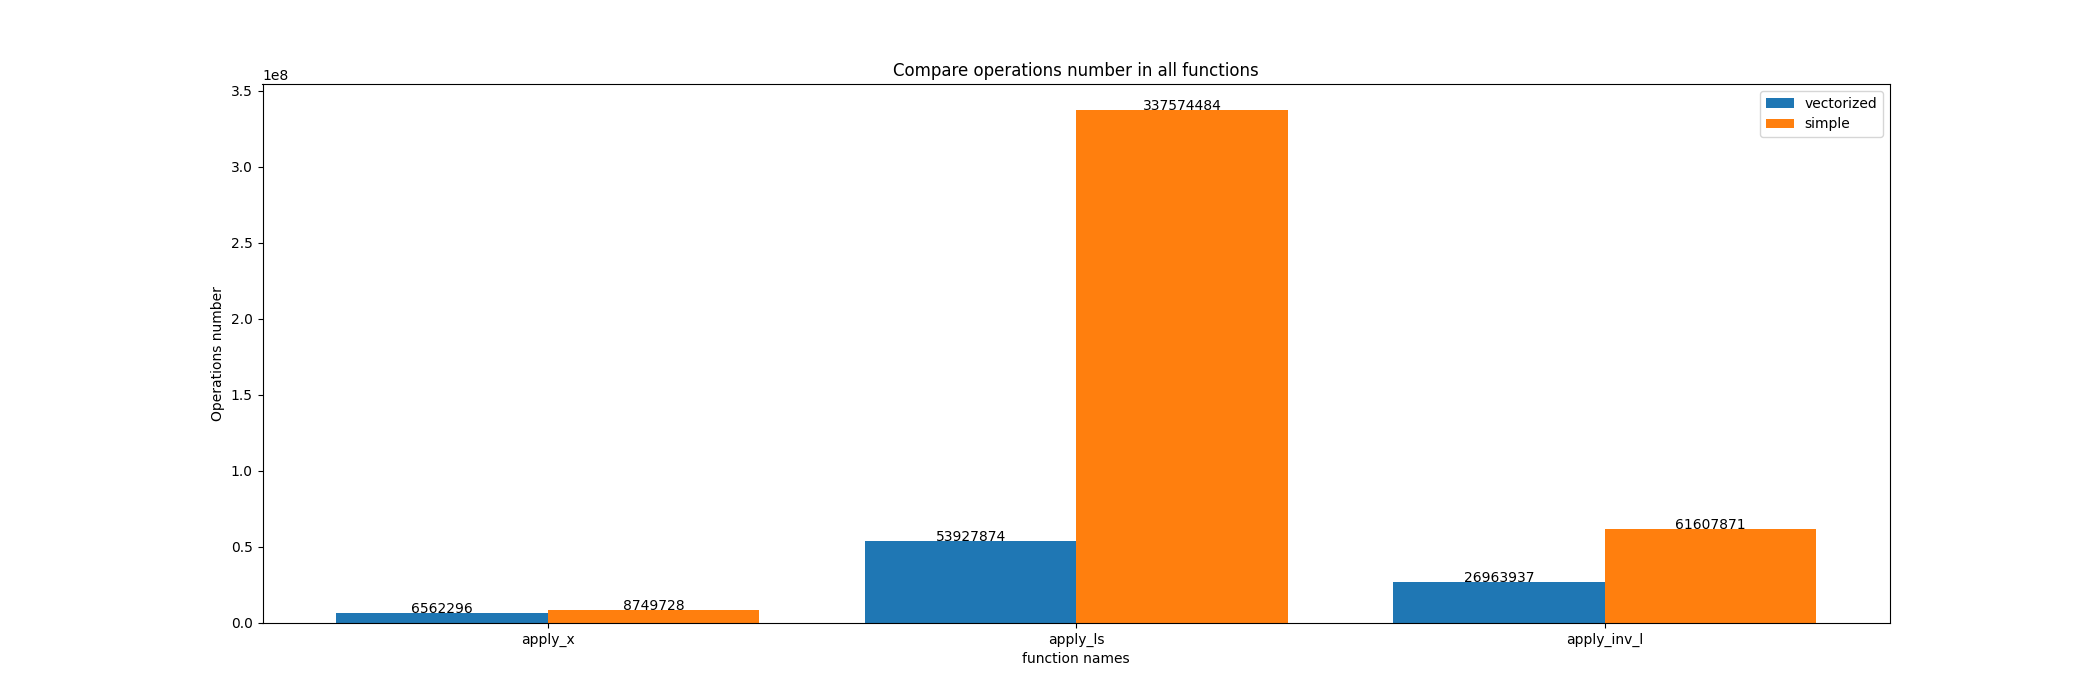
\includegraphics[scale=0.31]{images/functions_instructions_calls.png}
        \caption{Количество инструкций при вызове основных функций программы}
        \label{fig:functions_instructions_calls}
    \end{figure}

    \begin{figure}
        \centering
        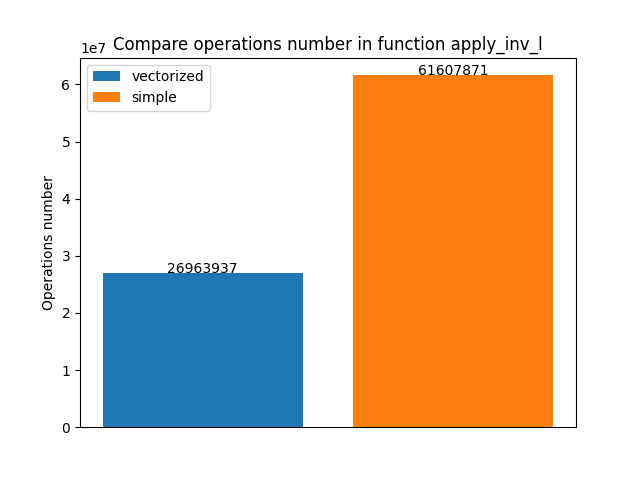
\includegraphics{images/one_function_innstructions_calls.png}
        \caption{Сравнение количества инструкций при вызове функции \text{apply\_inv\_l}}
        \label{fig:one_function_innstructions_calls}
    \end{figure}

    \begin{figure}
        \centering
        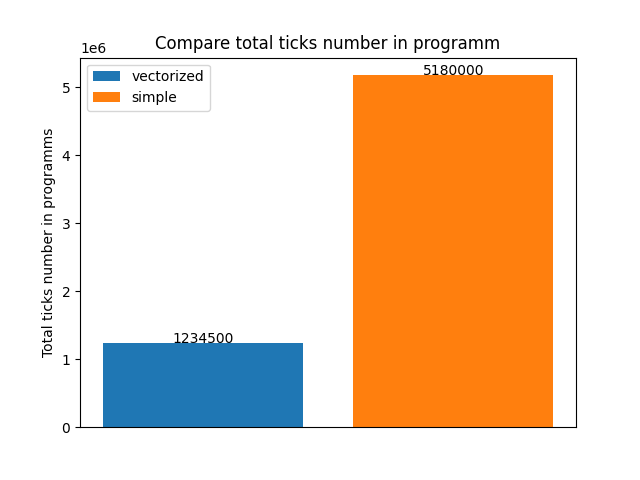
\includegraphics{images/total_ticks.png}
        \caption{Сравнение общего числа инструкций в программах}
        \label{fig:total_ticks}
    \end{figure}

    На рис. \ref{fig:functions_instructions_calls} изображены столбчатые 
    диаграммы, которые показывают количество инструкций для всех функций, имеющих векторную реализацию. Из графика видно, что на всех функциях векторизованная версия показала лучший результат.

    На рис. \ref{fig:one_function_innstructions_calls} изображен пример для одной функции.

    Кроме того, нам важно было получить уменьшение количества инструкций не только в рамках 
    конкретных функций, но и во всей программе в целом. На рис. \ref{fig:total_ticks} можно 
    увидеть полное число исполненных инструкций для наивной и 
    векторизованной версий.

    Итоговые результаты замеров продставленны в таблице \ref{tab:results}

    \begin{table}[]
    \begin{center}
    \begin{tabular}{|c|c|c|c|}
    \hline
    \textbf{Function} & Vectorized instruction count & Simple instruction count & Boost \\ \hline
    \texttt{apply\_x}          & $6562296$                      & $8749728$                  & $1.33$  \\ \hline
    \texttt{apply\_ls}         & $53927874$                     & $337574484$                & $6.26$  \\ \hline
    \texttt{apply\_inv\_l}     & $26963937$                     & $61607871$                 & $2.28$  \\ \hline
    Вся программа     & $1234500$                      & $518000$                   & $4.20$  \\ \hline
    \end{tabular}
    \end{center}
    \caption{Результаты измерений}
    \label{tab:results}
    \end{table}

    \section{Вывод}

    Таким образом в рамках нашей работы мы предложили корректную реализацию шифра 
    <<Кузнечик>>, а также привели высокопроизводительную версию этого шифра с 
    использованием инструкций из RVV spec 1.0. 
    
    Векторное расширение RISC-V позволяет получить прирост производительности без ухудшения масштабируемости кода даже для небольших программ.

\end{document}